\chapter{Combining Turing Machines}
\label{chap:combining}

In Chapter \ref{chap:definitions}, we have defined the notion of multi-tape Turing machines and basic machines.  In this chapter, we want to construct
more complex machines, for example a single-tape machine that moves the head to the right or to a certain symbol.
We define control flow operators, like ``match'', ``if then else'', ``sequential composition'', and ``while''.
As a result, we get a shallow-embed-ed language for programming multi-tape Turing machines in an imperative way.

\section{Match}
\label{sec:match}

Asperti and Ricciotti~\cite{asperti2015} also define the control flow operators sequential composition, conditional, and while.  However, for the
conditional they have to give one explicit ``else'' state.  Giving an explicit state is very tedious for complex machines.  That is why we use the
generalised notion of partitioned machines.  For example, for the conditional $\If{M_1}{M_2}{M_3}$, $M_1$ is partitioned over $\Bool$.  If $M_1$
terminated in a ``positive'' state (i.e. a state belonging to the partition $\true$), $M_2$ is executed after $M_1$.  Else it executes $M_3$ after
$M_1$.  We observe that sequential composition and conditional can be defined as instances of a more general operator we call $\MS{Match}$.  We give
proof scratches for the correctness and runtime in Subsection~\ref{sec:match-proofs}.

Let $M : \TM_\Sigma^n(F)$ and $M' \from F \to \TM_\Sigma^n(F')$ be a function from partitions to machines.  We define
$\MS{Match}~M~M' : \TM_\Sigma^n(F')$.

\begin{definition}[$\MS{Match}~M~M'$]
  \label{def:Match}
  \begin{alignat*}{3}
    & Q                  &~:=~& Q_M +  \sum_{y:F} Q_{M'(y)} \\
    & start              &~:=~& \inl start_M \\
    \delta ~&(\inl q, s) &~:=~&
    \begin{cases}
      \bigl(\inr (part_M~q, start_{M' (part_M~q)}), (\None, N)^n \bigr) & halt_M(q) \\
      \Let{(q', a) := \delta_M(q, s)}{\left(\inl q', a \right)} & \lnot halt_M(q)
    \end{cases} \\
    \delta ~&(\inr q, s) &~:=~& \Let{(q', a) := \delta_{M'(\pi_1 q)} (\pi_2 q, s)}{\bigl( \inr (\pi_1 q, q'), a \bigr)} \\
    halt   ~&(\inl  q)   &~:=~& \false \\
    halt   ~&(\inr  q)   &~:=~& halt_{M'(\pi_1~q)} (\pi_2~q) \\
    part   ~&(\inl  q)   &~:=~& \_ \\
    part   ~&(\inr  q)   &~:=~& part_{M'(\pi_1~q)} (\pi_2~q)
  \end{alignat*}
\end{definition}

In Definition~\ref{def:Match}, the $part$ value for $\inl$ is unimportant, because the states of $M_1$ are not terminating states.  We just use a
canonical value.

\begin{figure}
  \center
  \documentclass{standalone}

%%%
%%% Shared preamble for all files, e.g. thesis, TikZ standalones, slides, etc.
%%% It defines \macros for types, Turing machines, etc.
%%%

% Packages needed
\usepackage[utf8]{inputenc}
\usepackage{geometry}
\usepackage[small,compact]{titlesec}
\usepackage[final]{listings}
\usepackage{amsmath}
\usepackage[amsmath,hyperref,thmmarks]{ntheorem}
% Warning: The package ntheorem defines a \None macro!
\usepackage{amssymb}
\usepackage{tipa}
\usepackage[english]{babel}
\usepackage{lstautogobble}
\usepackage{proof}
\usepackage{bussproofs}
\usepackage{xparse}
\usepackage{needspace}
\usepackage{xspace}
\usepackage{mathpartir}
\usepackage{stmaryrd} % for |llbracket and \rrbracket
\usepackage{standalone} % useful to out-source graphics


% TikZ ist *kein* Zeichenprogramm.
\usepackage{tikz}
\usetikzlibrary{arrows,shapes,snakes,automata,backgrounds,fit,positioning}
\usepackage{tikz-cd} % for commutative diagrams


%% Formating
\newcommand{\MS}[1]{\ensuremath{\mathsf{#1}}}
\newcommand{\MST}[1]{${\mathsf{#1}}$}
\newcommand{\IsMathMode}{\ifmmode{This is math mode}\else{This is not math mode}\fi}

%% Logic symbols
\newcommand{\defop}{\mathop{:=}}
\newcommand{\imp}{\mathbin{\rightarrow}~}
\newcommand{\Imp}{\mathbin{\Rightarrow}~}
\renewcommand{\iff}{\mathbin{\leftrightarrow}}


% ++ operator:
% Source: https://tex.stackexchange.com/questions/4194/how-to-typeset-haskell-operator-and-friends
\newcommand\doubleplus{+\kern-1.3ex+\kern0.8ex}
\newcommand\mdoubleplus{\ensuremath{\mathbin{+\mkern-10mu+}}}
\newcommand{\app}{\mdoubleplus}

\newcommand{\rew}{\Rightarrow}
\newcommand{\trew}{\stackrel{\textrm{T}}\Rightarrow}
\newcommand{\llrew}{\stackrel{\textrm{L}}\Rightarrow}
\newcommand{\rlrew}{\stackrel{\textrm{R}}\Rightarrow}
\newcommand{\arew}{\triangleright}
\newcommand{\conc}{\mathop{{+}\hskip-5pt{+}}}
\newcommand{\gen}{\Rightarrow}

%% Sets
% \newcommand{\lam}[2]{\lambda#1{.}\hskip.7pt#2}
\newcommand{\setOf}[1]{\bigl\{ #1 \bigr \}}
\newcommand{\setMap}[2]{\setOf{#1~\big|~#2}}
\newcommand{\depPair}[2]{\setOf{#1~{\&}~#2}}
\newcommand{\pair}[2]{\bigl( #1 , #2 \bigr)}
\newcommand{\class}[1]{\bigl[ #1 \bigr]}
\newcommand{\choice}[1]{\bigl< #1 \bigr>}
\newcommand{\explainRel}[2]{\stackrel{\text{#1}}{#2}}
\newcommand{\family}[2]{\bigl( #1 \bigr)_{#2}}
\newcommand{\from}{:}
\renewcommand{\to}{\rightarrow}

%% Types
\newcommand{\Bool}{\mathbb{B}}
\newcommand{\Fin}{\mathbb{F}}
\newcommand{\Nat}{\mathbb{N}}
\newcommand{\Prop}{\mathbb{P}}
\newcommand{\Type}{\mathbb{T}}
\newcommand{\Unit}{\MS{1}}
\newcommand{\Option}{\mathcal{O}}
\newcommand{\List}{\mathcal{L}}
\newcommand{\Rel}{\MS{Rel}}

\newcommand{\True}{\top}
\newcommand{\False}{\bot}

%% Tapes
\newcommand{\tape}[1]{[ #1 ]}
\newcommand{\tapePointer}[1]{\underset{\uparrow}{#1}}
\newcommand{\niltape}{\tape{\tapePointer{}}}
\newcommand{\midtape}[3]{\tape{#1~\tapePointer{#2}~#3}}
\newcommand{\leftof}[2]{\tape{\tapePointer{}~#1~#2}}
\newcommand{\rightof}[2]{\tape{#1~#2~\tapePointer{}}}

% \newcommand{\niltape}{\MS{niltape}}
% \newcommand{\midtape}[3]{\MS{midtape}~#1~#2~#3}
% \newcommand{\leftof}[2]{\MS{leftof}~#1~#2}
% \newcommand{\rightof}[2]{\MS{rightof}~#1~#2}

%% Turing machine types
\newcommand{\Loop}{\MS{loop}}
\newcommand{\Tape}{\MS{Tape}}
\newcommand{\Tapes}[1]{\Tape^{#1}}
\newcommand{\TM}{\MS{TM}}
\newcommand{\Move}{\MS{Move}}
\newcommand{\Act}{\MS{Act}}
\newcommand{\Conf}{\MS{Conf}}
\newcommand{\Tau}{\Gamma}

%% Relations
\newcommand{\rif}{\mathbin{\phi}}
\newcommand{\at} [2][]{#1{|}_{#2}}
\newcommand{\att}[2][]{#1{|\mkern-1.5mu|}_{#2}}
\DeclareMathOperator{\ignoreParam}{\Uparrow}
\DeclareMathOperator{\hideParam}{\Downarrow}


%% Constructors
\DeclareMathOperator{\inl}{\ensuremath{\MS{inl}}}
\DeclareMathOperator{\inr}{\ensuremath{\MS{inr}}}
\newcommand{\Some}[1]{\left\lfloor {#1} \right\rfloor}
% \None is defined sometimes
\renewcommand{\None}{\emptyset}
\newcommand{\true}{\MS{true}}
\newcommand{\false}{\MS{false}}
\newcommand{\unit}{\MS{()}}
\newcommand{\nil}{\MS{nil}}
\newcommand{\cons}{\mathbin{::}}

%% Functions
\newcommand{\map}[2]{\ensuremath{\MS{map}~#1~#2}}
\newcommand{\maptwo}[3]{\ensuremath{\MS{map}_2~#1~#2~#3}}
\newcommand{\rev}[1]{\MS{rev}~#1}

%% Vector
\newcommand{\Vector}[1]{\left[ #1 \right]}
\DeclareMathOperator{\hd}{\ensuremath{\MS{hd}}}
\DeclareMathOperator{\tl}{\ensuremath{\MS{tl}}}
\newcommand{\length}[1]{\left| #1 \right|}
\newcommand{\blength}[1]{\bigl| #1 \bigr|}


%%
%% Encding
%%
\newcommand{\contains}{\simeq}
\newcommand{\size}[1]{\length{encode(#1)}}

%% Semantics
\newcommand{\terminates}{\mathrel{\triangleright}}
\newcommand{\TerminatesIn}{\mathrel{\downarrow}}
\newcommand{\Realise}{\mathrel{\vDash}}
\newcommand{\RealiseIn}[1]{\mathrel{\vDash^{#1}}}

%%
%% Turing Machines
%%

%% Control flow operators
\newcommand{\While}{\MS{While}}
\newcommand{\Seq}{;~}
\newcommand{\Match}{\MS{Match}}
\newcommand{\If}[3]{\MS{If}~#1~\MS{Then}~#2~\MS{Else}~#3}
\newcommand{\Let}[2]{\MS{let}~#1~\MS{in}~#2}
\newcommand{\cond}[3]{\MS{if}~#1~\MS{then}~#2~\MS{else}~#3}
\newcommand{\Nop}{\MS{Nop}}
\newcommand{\Return}[2]{\MS{Return}~#1~#2}
% \newcommand{\Return}[2]{\MS{Return}_{#2}~#1}

%% Lifts
% #1 is the machine, #2 the lifting
\newcommand{\LiftTapes}[2]{\mathop{\Uparrow_{#2}} #1}
\newcommand{\LiftAlphabet}[2]{\mathop{\Uparrow_{#2}} #1}
% #1 is the machine, #2 the alphabet lifting, and #3 the tape-lifting
\newcommand{\LiftBoth}[3]{\mathop{\Uparrow_{#2;~#3}} #1}




%%%
%%% lstlisting
%%%

% Style and language to define complex multi-line definitions similar to Coq code
\lstdefinelanguage{semicoq}{
  keywords={if,then,else,true,false,match,Match,If,Then,Else,Nop,Return,Move,Reset,DoAct,WriteMove,L,R,N},
  comment=[s]{(*}{*)},
}

%% Overlap #2 over phantom #1, e.g.
%% % XX\phalign{abcdefg}{YY}XX \\
%% % XXabcdefgXX
%% gets
%% XXYY     XX
%% XXabcdefgXX
%% Idea from https://tex.stackexchange.com/questions/212710/fill-space-created-by-phantom-with-other-text
\newcommand{\phalign}[2]{\makebox[0pt][l]{\ensuremath{#2}}\phantom{#1}}

\lstdefinestyle{semicoqstyle}{
  mathescape=true,
  keywordstyle=\textsf,
  language=semicoq,
  literate={
    {=>}{{$\Rightarrow$}}2
    {>->}{{$\rightarrowtail\,$}}2
    {<->}{{$\leftrightarrow$ }}2
    {->}{{$\to$ }}3
    {~}{{$\lnot$}}1
    {/\\}{{$\land$}}2
    {\\/}{{$\lor$}}2
    {forall}{{$\forall$}}1
    {exists}{{$\exists$}}1
    {<>}{{$\not =$}}{1}
    {<=}{{$\leq$}}{1}
    {<}{{$\lt$}}{1}
    {>=}{{$\ge$}}{1}
    {>}{{$\gt$}}{1}
    {[}{{$[$}}{1}
    {|}{{$|$}}{1}
    {]}{{$]$}}{1}
    {])}{{$])$}}{2}
    {(}{{$($}}{1}
    {)}{{$)$}}{1}
    {match}{{$\MS{match}$}}5
    {if}{{$\MS{if}$}}1
    {then}{{$\phalign{\MS{else}}{{\MS{then}}}$}}3
    {else}{{$\phalign{\MS{else}}{{\MS{else}}}$}}3
    {If}{{$\MS{If}$}}2
    {Then}{{$\phalign{\MS{Else}}{{\MS{Then}}}$}}4
    {Else}{{$\phalign{\MS{Else}}{{\MS{Else}}}$}}4
  }
}

\lstdefinelanguage{pseudocode}{
  keywords={If,Then,Else,Do,While,Reset,Return,Continue,Break},
}

\lstdefinestyle{pseudocode}{
  mathescape=true,
  language=pseudocode,
  literate={
    {:=}{{$\leftarrow$}}{2}
    {<>}{{$\not =$}}{1}
    {<=}{{$\leq$}}{1}
    {<}{{$\lt$}}{1}
    {>=}{{$\ge$}}{1}
    {>}{{$\gt$}}{1}
  }
}






%%% Local Variables:
%%% mode: LaTeX
%%% TeX-master: "thesis"
%%% End:

\begin{document}
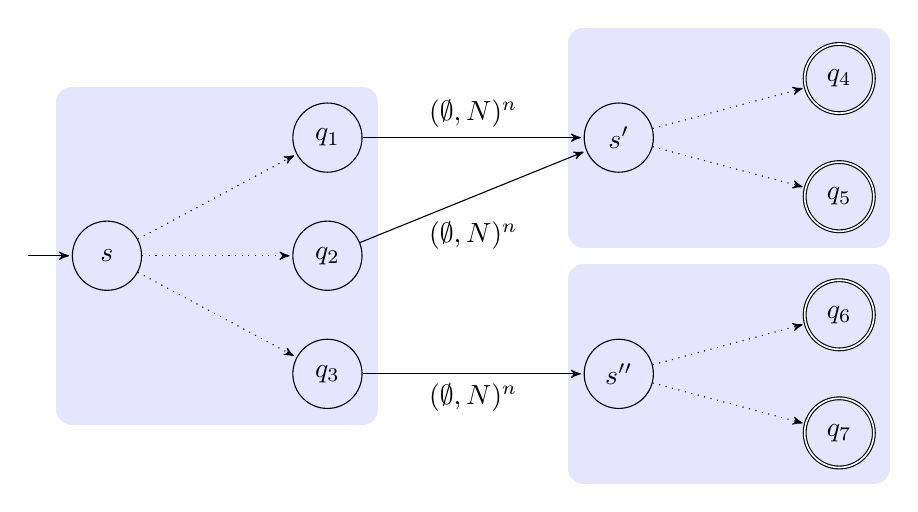
\begin{tikzpicture}[->,>=stealth',shorten >=1pt,auto,node distance=2.8cm]
  \begin{scope}
	  % Machine M
	  \node[state]          (M init)                                    {$s$};
	  \node[state]          (M exit 1)  [right of=M init,yshift= 1.5cm] {$q_1$};
	  \node[state]          (M exit 2)  [right of=M init,yshift= 0.0cm] {$q_2$};
	  \node[state]          (M exit 3)  [right of=M init,yshift=-1.5cm] {$q_3$};
	  \path (M init)
	  edge[dotted] (M exit 1)
	  edge[dotted] (M exit 2)
	  edge[dotted] (M exit 3);
	  \path (M init) ++(-1.0,0) edge (M init);
  \end{scope}
  \begin{scope}[xshift=6.5cm]
	  % Match-Machines
	  \begin{scope}[yshift=1.5cm]
		  % Accepting match machine
		  \node[state]          (M 1 init)                                        {$s'$};
		  \node[state, double]  (M 1 exit 1)  [right of=M 1 init, yshift= 0.75cm] {$q_4$};
		  \node[state, double]  (M 1 exit 2)  [right of=M 1 init, yshift=-0.75cm] {$q_5$};
		  \path (M 1 init)
		  edge[dotted] (M 1 exit 1)
		  edge[dotted] (M 1 exit 2);
	  \end{scope}
	  \begin{scope}[yshift=-1.5cm]
		  % Accepting match machine
		  \node[state]          (M 2 init)                                        {$s''$};
		  \node[state, double]  (M 2 exit 1)  [right of=M 2 init, yshift= 0.75cm] {$q_6$};
		  \node[state, double]  (M 2 exit 2)  [right of=M 2 init, yshift=-0.75cm] {$q_7$};
		  \path (M 2 init)
		  edge[dotted] (M 2 exit 1)
		  edge[dotted] (M 2 exit 2);
	  \end{scope}
  \end{scope}
  % Connecting edges
  \path
  (M exit 1) edge node[anchor=south] {$(\emptyset, N)^n$} (M 1 init)
  (M exit 2) edge node[anchor=north,yshift=-0.2cm] {$(\emptyset, N)^n$} (M 1 init)
  (M exit 3) edge node[anchor=north] {$(\emptyset, N)^n$} (M 2 init);

  \begin{pgfonlayer}{background}
	  \filldraw [line width=4mm,join=round,blue!10]
	  (M   exit 1.north -| M   init.west) rectangle (M   exit 3.south -| M   exit 3.east)
	  (M 1 exit 1.north -| M 1 init.west) rectangle (M 1 exit 2.south -| M 1 exit 2.east)
	  (M 2 exit 1.north -| M 2 init.west) rectangle (M 2 exit 2.south -| M 2 exit 2.east);
  \end{pgfonlayer}
\end{tikzpicture}

\end{document}


%%% Local Variables:
%%% TeX-master: t
%%% End:
  \caption{Example of a $\MS{Match}$.  The left box stands for the first machine $M_1:\TM_\Sigma^n(\Bool)$.  The states $q_1$ and $q_2$ are mapped to
    $\true$, $q_3$ is mapped to $\false$.  After the $\MS{Match}$ reaches one of the injections of the terminal states $q_1, \cdots, q_3$ of $M_1$, it
    continues its execution either in the top case machine $M_2$ or in the bottom case machine $M_3$.  The halting states of $\MS{Match}$ are exactly
    the injections of the halting states of the case-machines.}
  \label{fig:match}
\end{figure}

\todo{Maybe use parenthesises, e.g.\ $\Match(M,M')$ and $\MS{MatchRel}(R,R')$ for better readability}


$\MS{Match}~M~M'$ first executes a copy of $M$.  When it reaches a final state $q$ of $M$, it does a ``nop'' action (i.e.\ $(\None,N)^n$) and changes
to to the injection of the start state of the machine $M'(part~q)$.  When $\MS{Match}~M~M'$ reaches a state that is the injection of a final state of
a machine $M'~y$, it terminates.  The correctness part of the semantics can be expressed using the following lemma:

\begin{lemma}[Correctness of $\MS{Match}~M~M'$]
  \label{lem:Match_Realise}
  Let $R \subseteq \Tape_\Sigma^n \times F \times \Tape_\Sigma^n$ and $R'~y \subseteq \Tape_\Sigma^n \times F' \times \Tape_\Sigma^n$ for all $y:F$.
  If $M \vDash R$ and $M'~y \vDash R'~y$ for all $y:F$, then
  \[
    \MS{Match}~M~M' \vDash \MS{MatchRel}~R~R'
  \]
  with
  \[
    \MS{MatchRel}~R~R' := \bigcup_{y:F} \bigl( R\at y \circ R'~y \bigr).
  \]
\end{lemma}

Note that in the relation $\MS{MatchRel}$, we compose the unpartitioned relation $R \at y \subseteq \Tape_\Sigma^n \times \Tape_\Sigma^n$ with the
partitioned relation $R'~y \subseteq \Tape_\Sigma^n \times F' \times \Tape_\Sigma^n$.  This means that $\Match~M~M'$ ``discards'' the partition of the
final state of $M$ and terminates in the partition of $M'~y$.

To specify the runtime of $\MS{Match}~M~M'$, we need to know the runtime relation in that $M$ terminates, and for each $y:F$ the runtime of $M'~y$.
We also need to know the correctness of $M$, because the runtime of $M'~y$ depends on the output of $M$, which is the input of $M~y$.

\begin{lemma}[Runtime of $\MS{Match}~M~M'$]
  \label{lem:Match_Terminates}
  Let $R \subseteq \Tape_\Sigma^n \times F \times \Tape_\Sigma^n$, $T \subseteq \Tape_\Sigma^n \times \Nat$, and
  $T'~y \subseteq \Tape_\Sigma^n \times \Nat$ for all $y:F$.  If $M \vDash R$, $M \downarrow T$, and $M'~y \downarrow T'~y$ for all $y:F$, then
  $\MS{Match}~M~M' \downarrow \MS{MatchT}~R~T~T'$, where
  \[
    \MS{MatchT}~R~T~T' :=
    \lambda~t~i.~ \exists~i_1~i_2.~T~t~i_1 \land 1+i_1+i_2 \le i \land
      \forall~y~t'.~ R~t~y~t' \rightarrow T'~y~t'~i_2
  \]
\end{lemma}


\subsection{Derived Operators}
\label{sec:match-derived-operators}

As mentioned above, conditional and sequential composition can be defined as instances of the Match operator.  For the conditional
$\If{M_1}{M_2}{M_3}$ with $M_1 : \TM_\Sigma^n(\Bool)$, $M_2, M_3 : \TM_\Sigma^n(F')$, $f$ simply maps $\true$ to $M_2$ and $\false$ to $M_3$.  For the
sequential composition $M_1 \Seq M_2$ with $M_1 : \TM_\Sigma^n(F)$ and $M_2 : \TM_\Sigma^n(F')$, $f$ maps all partitions of $F$ to $M_2$.

\begin{definition}[Conditional]
  \label{def:If}
  Let $M_1 : \TM_\Sigma^n(\Bool)$, $M_2, M_3 : \TM_\Sigma^n(F')$.
  \[
    \If{M_1}{M_2}{M_3} := \Match~M_1~
    \left(\lam{b}{\cond{b}{M_2}{M_3} \right})
  \]
\end{definition}

\begin{definition}[Sequencial composition]
  Let $M_1 : \TM_\Sigma^n(F)$ and $M_2 : \TM_\Sigma^n(F')$ .
  \[
    M_1 \Seq M_2 := \Match~M_1~
    \bigl(
    \lambda~\_.~M_2
    \bigr)
  \]
\end{definition}


\subsection{Proof of $\Match$}
\label{sec:match-proofs}

The idea of the proofs of Lemma~\ref{lem:Match_Realise} and Lemma~\ref{lem:Match_Terminates} is to abstract two features of the machine: lifting of
configurations from one abstract machine to another abstract machines and sequence of two loops.  We formalise these two concepts for abstract
machines, i.e.\ we argue on the abstract $\Loop$ function.

For the first feature, \emph{lifting}, we assume two types $A$, $B$ for abstract configurations, an injective function $lift : A \to B$, two step
functions $f : A \to A$, $f' : B \to B$, and two halting function $h : A \to \Bool$, $h' : B \to \Bool$.  We assume that the step functions $f$ and
$f'$, which are compatible with $lift$ in non-halting states of $A$.  Formally, this means
\begin{equation}
  \label{eq:loop_lift_assumption1}
  \forall a:A.~\lnot h~x \rightarrow f' (lift~x) = lift (f~x).
\end{equation}

The second assumptions is that $h'$ is compatible with $h$, w.r.t.\ $lift$, formally:
\begin{equation}
  \label{eq:loop_lift_assumption2}
  \forall a:A.~h'(lift~x)=h~x.
\end{equation}

Under these two assumptions we can show two lemmas that essentially say that the second abstract machine $B$ simulates the first machine $A$.
\begin{lemma}[Loop lifting]
  \label{lem:loop_lift}
  Under the assumptions~\ref{eq:loop_lift_assumption1} and~\ref{eq:loop_lift_assumption2}:
  \begin{alignat*}{1}
    & \forall (k:\Nat)~(c_1~c_2 : A). \\
    & \quad \Loop~f ~h ~k~c_1 = \Some{c_2} \rightarrow \\
    & \quad \Loop~f'~h'~k~(lift~c_1) = \Some {lift~c_2}
  \end{alignat*}
\end{lemma}
\begin{proof}
  By induction over $k:\Nat$.
\end{proof}
\begin{lemma}[Loop unlifting]
  \label{lem:loop_unlift}
  Under the assumptions~\ref{eq:loop_lift_assumption1} and~\ref{eq:loop_lift_assumption2}:
  \begin{alignat*}{1}
    & \forall (k:\Nat)~(a:A)~(b':B). \\
    & \quad \Loop~f'~h'~k~(lift~a) = \Some{b'} \rightarrow \\
    & \quad \exists (b:B).~\Loop~f~h~k~a = \Some b \land b'=lift~b
  \end{alignat*}
\end{lemma}
\begin{proof}
  By induction over $k:\Nat$.
\end{proof}

For the second feature, \emph{sequencing}, we assume a type $A$ with the step function $f \from A \to A$ and two halting functions
$h \from A \to \Bool$ and $h' \from A \to \Bool$.  We assume
\begin{equation}
  \label{eq:loop_merge_assumption}
  \forall(a:A).~h~a = \false \rightarrow h'~a = \false,
\end{equation}
i.e.\ either $a$ is a halting state w.r.t.\ $h'$, or $a$ is a non-halting state w.r.t.\ $h$.
\begin{lemma}[Loop merging]
  \label{lem:loop_merge}
  Under assumption~\ref{eq:loop_merge_assumption}:
  \begin{align*}
    & \forall (k_1~k_2:\Nat)~(c_1~c_2~c_3 : A).\\
    & \quad \Loop~f~h ~k_1      ~c_1 = \Some{c_2} \rightarrow\\
    & \quad \Loop~f~h'~k_2      ~c_2 = \Some{c_3} \rightarrow\\
    & \quad \Loop~f~h'~(k_1+k_2)~c_1 = \Some{c_3}.
  \end{align*}
\end{lemma}
\begin{proof}
  By induction over $k_1:\Nat$, using Lemma~\ref{lem:loop}~(\ref{lem:loop_monotone}).
\end{proof}
\begin{lemma}[Loop splitting]
  \label{lem:loop_split}
  Under the above assumption:
  \begin{align*}
    & \forall (k:\Nat)~(c_1~c_3 : A).\\
    & \quad \Loop~f~h'~k~c_1 = \Some{c_3} \rightarrow \\
    & \quad \exists (k_1~k_2:\Nat)~(c_2:A).\\
    & \quad \quad \Loop~f~h~k_1~c_1 = \Some{c_2} \land\\
    & \quad \quad \Loop~f~h~k_2~c_2 = \Some{c_3} \land\\
    & \quad \quad k_1 + k_2 \leq k.
  \end{align*}
\end{lemma}
\begin{proof}
  By complete induction over $k:\Nat$.
\end{proof}


Back to the verification of $\Match~M~M'$.  In the following, we simply write $\Match$.  The execution steps of $\Match$ are essentially a sequence of
first, the lifted steps of execution of $M$, second, a ``nop'' transition, and third, the lifted steps of the execution of $M'~y$.  We give the
concrete lifting functions from $M$ to $\Match$ and from $M~y$ to $\Match$:
\begin{definition}[Liftings of $\Match$]
  We define the functions \\$liftL : \Conf_M \to \Conf_\Match$ and $liftR_y : \Conf_{M'~y} \to \Conf_\Match$:
  \begin{alignat*}{2}
    & liftL   & (q, t) &:= (\inl q,      t) \\
    & liftR_y & (q, t) &:= (\inr (y, q), t).
  \end{alignat*}
\end{definition}

For the sequential part, we also have to define the lifted halting function of \\$haltConfL : \Conf_\Match \to \Bool$:
\begin{definition}[Lifted halting function]
  \begin{alignat*}{2}
    & haltConfL & (\inl~q, t) &:= halt_M(q) \\
    & haltConfL & (\inr~q, t) &:= \true
  \end{alignat*}
\end{definition}

Using Lemma \ref{lem:loop_merge} and \ref{lem:loop_lift}, we can show the lemma we need for runtime:
\begin{lemma}[Merging parts of executions of $\Match$]
  \label{lem:Match_merge}
  Let $t : \Tape_\Sigma^n$, $k_1, k_2:\Nat$, $c_1=(q', t') : \Conf_M$ and $c_2=(q'', t'') : \Conf_{M'~y}$.
  \begin{alignat*}{1}
    & M(t) \terminates^{k_1} c_1 \rightarrow\\
    & \bigl( M'~(part_M~q') \bigr) (t_1) \terminates^{k_2} c_2 rightarrow\\
    & \Match(t) \terminates^{1+k_1+k_2} liftR(c_2).
  \end{alignat*}
\end{lemma}
\begin{proof}
  We apply \ref{lem:loop_merge} and have to show:
  \begin{enumerate}
  \item $\forall a:\Conf_\Match.~ \lnot haltConfL~a \rightarrow \lnot \MS{haltConf}~a$.  This holds trivially by definition.
  \item $loop~k_1~step_\Match~haltConfL~(\MS{initConf}_\Match~t) =
    \Some{liftL~c1}$.  By definition, we have $\MS{initConf}_\Match~t=liftL(\MS{initConf}_M t)$.  The claim follows with Lemma~\ref{lem:loop_lift}.
  \item $loop~(1+k_2)~step_\Match~haltConf_\Match~(liftL~c1) =
    \Some{liftR(c_2)}$.  By definition, we know that the first step must be a ``nop'' transition from
    $liftL~c_1$ to $liftR~\bigl(\MS{initConf}_{M'(part_M~q')}~t' \bigr)$.
    It remains to show that
    $$ loop~k_2~step_\Match~haltConf_\Match~liftR \bigl(\MS{initConf}_{M'(part_M~q')}~t' \bigr) = liftR(c_2).$$
    This follows with Lemma~\ref{lem:loop_merge}.
  \end{enumerate}
\end{proof}
The runtime Lemma~\ref{lem:Match_Terminates} follows directly from Lemma~\ref{lem:Match_merge}.

\begin{lemma}[Splitting execution of $\Match$]
  \label{lem:Match_split}
  Let $t : \Tape_\Sigma^n$, $k : \Nat$, $c : \Conf_\Match$.
  \begin{align*}
    & \Match(t) \terminates^k outc \rightarrow \\
    & \exists (k_1~k_2 : \Nat)~(c_1 = (q', t') : \Conf_M)~(c_2 : \Conf_{M'(part_M~q')}). \\
    & \quad M(t) \terminates^{k_1} c_1 ~\land~ \\
    & \quad \bigl( M' (part_M~q') \bigr) (t') \terminates^{k_2} c_2 ~\land~ \\
    & \quad c = liftR(c_2).
  \end{align*}
\end{lemma}
\begin{proof}
  Analogous to the proof of Lemma~\ref{lem:Match_merge}, using Lemma~\ref{lem:loop_split} and Lemma~\ref{lem:loop_unlift}.
\end{proof}
The correctness Lemma~\ref{lem:Match_Realise} follows directly from Lemma~\ref{lem:Match_split}.


Asperti and Ricciotti~\cite{asperti2015} have a version of Lemma~\ref{lem:loop_lift} and Lemma~\ref{lem:loop_merge}.

\section{While}
\label{sec:While}


The machine $\While M$ essentially behaves like a ``do-while'' loop in imperative languages like C.  At the end of the execution of the loop body $M$,
$M$ decides either to continue or break out of the loop.  If $M$ terminated in the partition $\None$, then the loop is continued, and if $M$ terminated
in $\Some{y}$, the loop brakes and $\While M$ terminates in $y$.  When $M : \TM_\Sigma^n(\Option(F))$, then $\While M : \TM_\Sigma^n(F)$.

\begin{definition}[$\MS{While}~M$]
  \label{def:While}
  Let $M : \TM_\Sigma^n(\Option(F))$ and $def:F$.
  \begin{alignat*}{3}
    & F              &~:=~& F \\
    & Q              &~:=~& Q_M \\
    & start          &~:=~& start_M \\
    \delta ~& (q, s) &~:=~&
    \begin{cases}
      (q,       (\None, N)^n) & halt_M(q) \land part_M(q) = \Some y \\
      (start_M, (\None, N)^n) & halt_M(q) \land part_M(q) = \None \\
      \delta_M (q,s)    & \lnot halt_M(q)
    \end{cases} \\
    halt ~& q      &~:=~& halt_M(q) \land \MS{isSome}(part_M(q)) \\
    part ~& q      &~:=~&
    \begin{cases}
      y   & part_M(q) = \Some y \\
      def & part_M(q) = \None
    \end{cases}
  \end{alignat*}
\end{definition}

\begin{figure}
  \center
  \documentclass{standalone}

%%%
%%% Shared preamble for all files, e.g. thesis, TikZ standalones, slides, etc.
%%% It defines \macros for types, Turing machines, etc.
%%%

% Packages needed
\usepackage[utf8]{inputenc}
\usepackage{geometry}
\usepackage[small,compact]{titlesec}
\usepackage[final]{listings}
\usepackage{amsmath}
\usepackage[amsmath,hyperref,thmmarks]{ntheorem}
% Warning: The package ntheorem defines a \None macro!
\usepackage{amssymb}
\usepackage{tipa}
\usepackage[english]{babel}
\usepackage{lstautogobble}
\usepackage{proof}
\usepackage{bussproofs}
\usepackage{xparse}
\usepackage{needspace}
\usepackage{xspace}
\usepackage{mathpartir}
\usepackage{stmaryrd} % for |llbracket and \rrbracket
\usepackage{standalone} % useful to out-source graphics


% TikZ ist *kein* Zeichenprogramm.
\usepackage{tikz}
\usetikzlibrary{arrows,shapes,snakes,automata,backgrounds,fit,positioning}
\usepackage{tikz-cd} % for commutative diagrams


%% Formating
\newcommand{\MS}[1]{\ensuremath{\mathsf{#1}}}
\newcommand{\MST}[1]{${\mathsf{#1}}$}
\newcommand{\IsMathMode}{\ifmmode{This is math mode}\else{This is not math mode}\fi}

%% Logic symbols
\newcommand{\defop}{\mathop{:=}}
\newcommand{\imp}{\mathbin{\rightarrow}~}
\newcommand{\Imp}{\mathbin{\Rightarrow}~}
\renewcommand{\iff}{\mathbin{\leftrightarrow}}


% ++ operator:
% Source: https://tex.stackexchange.com/questions/4194/how-to-typeset-haskell-operator-and-friends
\newcommand\doubleplus{+\kern-1.3ex+\kern0.8ex}
\newcommand\mdoubleplus{\ensuremath{\mathbin{+\mkern-10mu+}}}
\newcommand{\app}{\mdoubleplus}

\newcommand{\rew}{\Rightarrow}
\newcommand{\trew}{\stackrel{\textrm{T}}\Rightarrow}
\newcommand{\llrew}{\stackrel{\textrm{L}}\Rightarrow}
\newcommand{\rlrew}{\stackrel{\textrm{R}}\Rightarrow}
\newcommand{\arew}{\triangleright}
\newcommand{\conc}{\mathop{{+}\hskip-5pt{+}}}
\newcommand{\gen}{\Rightarrow}

%% Sets
% \newcommand{\lam}[2]{\lambda#1{.}\hskip.7pt#2}
\newcommand{\setOf}[1]{\bigl\{ #1 \bigr \}}
\newcommand{\setMap}[2]{\setOf{#1~\big|~#2}}
\newcommand{\depPair}[2]{\setOf{#1~{\&}~#2}}
\newcommand{\pair}[2]{\bigl( #1 , #2 \bigr)}
\newcommand{\class}[1]{\bigl[ #1 \bigr]}
\newcommand{\choice}[1]{\bigl< #1 \bigr>}
\newcommand{\explainRel}[2]{\stackrel{\text{#1}}{#2}}
\newcommand{\family}[2]{\bigl( #1 \bigr)_{#2}}
\newcommand{\from}{:}
\renewcommand{\to}{\rightarrow}

%% Types
\newcommand{\Bool}{\mathbb{B}}
\newcommand{\Fin}{\mathbb{F}}
\newcommand{\Nat}{\mathbb{N}}
\newcommand{\Prop}{\mathbb{P}}
\newcommand{\Type}{\mathbb{T}}
\newcommand{\Unit}{\MS{1}}
\newcommand{\Option}{\mathcal{O}}
\newcommand{\List}{\mathcal{L}}
\newcommand{\Rel}{\MS{Rel}}

\newcommand{\True}{\top}
\newcommand{\False}{\bot}

%% Tapes
\newcommand{\tape}[1]{[ #1 ]}
\newcommand{\tapePointer}[1]{\underset{\uparrow}{#1}}
\newcommand{\niltape}{\tape{\tapePointer{}}}
\newcommand{\midtape}[3]{\tape{#1~\tapePointer{#2}~#3}}
\newcommand{\leftof}[2]{\tape{\tapePointer{}~#1~#2}}
\newcommand{\rightof}[2]{\tape{#1~#2~\tapePointer{}}}

% \newcommand{\niltape}{\MS{niltape}}
% \newcommand{\midtape}[3]{\MS{midtape}~#1~#2~#3}
% \newcommand{\leftof}[2]{\MS{leftof}~#1~#2}
% \newcommand{\rightof}[2]{\MS{rightof}~#1~#2}

%% Turing machine types
\newcommand{\Loop}{\MS{loop}}
\newcommand{\Tape}{\MS{Tape}}
\newcommand{\Tapes}[1]{\Tape^{#1}}
\newcommand{\TM}{\MS{TM}}
\newcommand{\Move}{\MS{Move}}
\newcommand{\Act}{\MS{Act}}
\newcommand{\Conf}{\MS{Conf}}
\newcommand{\Tau}{\Gamma}

%% Relations
\newcommand{\rif}{\mathbin{\phi}}
\newcommand{\at} [2][]{#1{|}_{#2}}
\newcommand{\att}[2][]{#1{|\mkern-1.5mu|}_{#2}}
\DeclareMathOperator{\ignoreParam}{\Uparrow}
\DeclareMathOperator{\hideParam}{\Downarrow}


%% Constructors
\DeclareMathOperator{\inl}{\ensuremath{\MS{inl}}}
\DeclareMathOperator{\inr}{\ensuremath{\MS{inr}}}
\newcommand{\Some}[1]{\left\lfloor {#1} \right\rfloor}
% \None is defined sometimes
\renewcommand{\None}{\emptyset}
\newcommand{\true}{\MS{true}}
\newcommand{\false}{\MS{false}}
\newcommand{\unit}{\MS{()}}
\newcommand{\nil}{\MS{nil}}
\newcommand{\cons}{\mathbin{::}}

%% Functions
\newcommand{\map}[2]{\ensuremath{\MS{map}~#1~#2}}
\newcommand{\maptwo}[3]{\ensuremath{\MS{map}_2~#1~#2~#3}}
\newcommand{\rev}[1]{\MS{rev}~#1}

%% Vector
\newcommand{\Vector}[1]{\left[ #1 \right]}
\DeclareMathOperator{\hd}{\ensuremath{\MS{hd}}}
\DeclareMathOperator{\tl}{\ensuremath{\MS{tl}}}
\newcommand{\length}[1]{\left| #1 \right|}
\newcommand{\blength}[1]{\bigl| #1 \bigr|}


%%
%% Encding
%%
\newcommand{\contains}{\simeq}
\newcommand{\size}[1]{\length{encode(#1)}}

%% Semantics
\newcommand{\terminates}{\mathrel{\triangleright}}
\newcommand{\TerminatesIn}{\mathrel{\downarrow}}
\newcommand{\Realise}{\mathrel{\vDash}}
\newcommand{\RealiseIn}[1]{\mathrel{\vDash^{#1}}}

%%
%% Turing Machines
%%

%% Control flow operators
\newcommand{\While}{\MS{While}}
\newcommand{\Seq}{;~}
\newcommand{\Match}{\MS{Match}}
\newcommand{\If}[3]{\MS{If}~#1~\MS{Then}~#2~\MS{Else}~#3}
\newcommand{\Let}[2]{\MS{let}~#1~\MS{in}~#2}
\newcommand{\cond}[3]{\MS{if}~#1~\MS{then}~#2~\MS{else}~#3}
\newcommand{\Nop}{\MS{Nop}}
\newcommand{\Return}[2]{\MS{Return}~#1~#2}
% \newcommand{\Return}[2]{\MS{Return}_{#2}~#1}

%% Lifts
% #1 is the machine, #2 the lifting
\newcommand{\LiftTapes}[2]{\mathop{\Uparrow_{#2}} #1}
\newcommand{\LiftAlphabet}[2]{\mathop{\Uparrow_{#2}} #1}
% #1 is the machine, #2 the alphabet lifting, and #3 the tape-lifting
\newcommand{\LiftBoth}[3]{\mathop{\Uparrow_{#2;~#3}} #1}




%%%
%%% lstlisting
%%%

% Style and language to define complex multi-line definitions similar to Coq code
\lstdefinelanguage{semicoq}{
  keywords={if,then,else,true,false,match,Match,If,Then,Else,Nop,Return,Move,Reset,DoAct,WriteMove,L,R,N},
  comment=[s]{(*}{*)},
}

%% Overlap #2 over phantom #1, e.g.
%% % XX\phalign{abcdefg}{YY}XX \\
%% % XXabcdefgXX
%% gets
%% XXYY     XX
%% XXabcdefgXX
%% Idea from https://tex.stackexchange.com/questions/212710/fill-space-created-by-phantom-with-other-text
\newcommand{\phalign}[2]{\makebox[0pt][l]{\ensuremath{#2}}\phantom{#1}}

\lstdefinestyle{semicoqstyle}{
  mathescape=true,
  keywordstyle=\textsf,
  language=semicoq,
  literate={
    {=>}{{$\Rightarrow$}}2
    {>->}{{$\rightarrowtail\,$}}2
    {<->}{{$\leftrightarrow$ }}2
    {->}{{$\to$ }}3
    {~}{{$\lnot$}}1
    {/\\}{{$\land$}}2
    {\\/}{{$\lor$}}2
    {forall}{{$\forall$}}1
    {exists}{{$\exists$}}1
    {<>}{{$\not =$}}{1}
    {<=}{{$\leq$}}{1}
    {<}{{$\lt$}}{1}
    {>=}{{$\ge$}}{1}
    {>}{{$\gt$}}{1}
    {[}{{$[$}}{1}
    {|}{{$|$}}{1}
    {]}{{$]$}}{1}
    {])}{{$])$}}{2}
    {(}{{$($}}{1}
    {)}{{$)$}}{1}
    {match}{{$\MS{match}$}}5
    {if}{{$\MS{if}$}}1
    {then}{{$\phalign{\MS{else}}{{\MS{then}}}$}}3
    {else}{{$\phalign{\MS{else}}{{\MS{else}}}$}}3
    {If}{{$\MS{If}$}}2
    {Then}{{$\phalign{\MS{Else}}{{\MS{Then}}}$}}4
    {Else}{{$\phalign{\MS{Else}}{{\MS{Else}}}$}}4
  }
}

\lstdefinelanguage{pseudocode}{
  keywords={If,Then,Else,Do,While,Reset,Return,Continue,Break},
}

\lstdefinestyle{pseudocode}{
  mathescape=true,
  language=pseudocode,
  literate={
    {:=}{{$\leftarrow$}}{2}
    {<>}{{$\not =$}}{1}
    {<=}{{$\leq$}}{1}
    {<}{{$\lt$}}{1}
    {>=}{{$\ge$}}{1}
    {>}{{$\gt$}}{1}
  }
}






%%% Local Variables:
%%% mode: LaTeX
%%% TeX-master: "thesis"
%%% End:

\begin{document}

  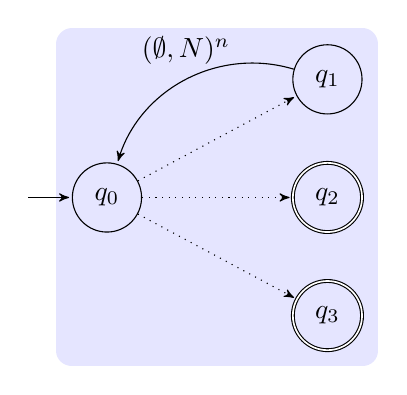
\begin{tikzpicture}[->,>=stealth',shorten >=1pt,auto,node distance=2.8cm,bend angle=45]
    \begin{scope}
      % Machine M
      \node[state]          (M init)                                    {$q_0$};
      \node[state]          (M exit 1)  [right of=M init,yshift= 1.5cm] {$q_1$};
      \node[state, double]  (M exit 2)  [right of=M init,yshift= 0.0cm] {$q_2$};
      \node[state, double]  (M exit 3)  [right of=M init,yshift=-1.5cm] {$q_3$};
      \path (M init)
      edge[dotted]          (M exit 1)
      edge[dotted]  (M exit 2)
      edge[dotted]  (M exit 3);
      \path (M init) ++(-1.0,0) edge (M init);
      \path (M exit 1) edge[bend right] node[anchor=south,yshift=0.2em] {$(\None, N)^n$} (M init);
    \end{scope}

    \begin{pgfonlayer}{background}
      \filldraw [line width=4mm,join=round,blue!10]
      (M   exit 1.north -| M   init.west) rectangle (M   exit 3.south -| M   exit 3.east);
    \end{pgfonlayer}
  \end{tikzpicture}

\end{document}

%%% Local Variables:
%%% TeX-master: t
%%% End:
  \caption{Example for $\While~M$ with $M:\TM_\Sigma^n(\Option(\Bool))$.  When the $M$ reaches the state $q_1$, the loop is continued, because $q_1$
    is in the partition $\None$ of $M$.  $q_2$ and $q_3$ are in the partition $\Some{\true}$ and $\Some{\false}$.  Therefore $\While~M$ terminates in
    its partition $\true$ or $\false$, when $M$ terminated in $q_2$ or $q_3$.}
  \label{fig:while-example}
\end{figure}

In Definition~\ref{def:While}, we have to assume that $F$ is inhabited.  However, the choice of $def:F$ is semantically irrelevant, because $\While~M$
only halts in states where $part_M(q)$ has a $\Some{.}$ value.

The correctness of $\MS{While}$ can be easily expressed using the following relation:

\begin{definition}[$WhileRel$]
\end{definition}

\begin{lemma}[Correctness of $\MS{While}$]
  \label{lem:While_Realise}
  Let $R \subseteq \Tape_\Sigma^n \times \Option(F) \times \Tape_\Sigma^n$.
  If $M \vDash R$, then $\While~M \vDash \MS{WhileRel}~M$, where
  $WhileRel~R \subseteq \Tape_\Sigma^n \times F \times \Tape_\Sigma^n$
  is inductively defined by the following two rules:
  \[
    \inferrule{R~t~(\None, t') \and WhileRel~R~t'~(y, t'')}{WhileRel~R~t~(y, t'')}
    \quad
    \inferrule{R~t~(\Some y, t')}{WhileRel~R~t~(y, t')}
  \]
\end{lemma}

We can also express the correctness relation of $\While$ using the Kleene star:
\begin{lemma}[Alternative specification of $\While~M$]
  ~
  \[
    \MS{WhileRel}~R \equiv (R \at \None)^* \circ \Bigl( \bigcup_{y:F} \bigl( R \at {\Some y} \bigr) \att y \Bigr)
  \]
\end{lemma}

Both definitions of $WhileRel$ should make clear what $\While~M$ does: It repeats the execution of $M$ as long as it terminated in $\None$, and
after it terminated in $\Some y$, it terminates in the partition $y$.  This is visualised in Figure~\ref{fig:while-example}.  However, the inductive
definition is more practical when we prove correctness of concrete $\MS{While}$ machines, because we can just do induction on the inductive predicate.

When we want to prove $\While~M \vDash R$ for some machine $M:\TM_\Sigma^n(F)$ and relation
$R \subseteq \Tape_\Sigma^n \times F \times \Tape_\Sigma^n$, we must of course have proven that $M \vDash R'$ for some relation
$R' \subseteq \Tape_\Sigma^n \times \Option(F) \times \Tape_\Sigma^n$.  Then we apply Lemma~\ref{lem:Realise_monotone} and~\ref{lem:While_Realise},
and have to show $WhileRel~R' \subseteq R$.  We can prove this by induction on the inductive predicate, which is equivalent to applying the following
lemma:
\begin{lemma}[Induction for $WhileRel$]
  \label{lem:WhileInduction}
  ~
  \begin{alignat*}{1}
    & \left(\forall t~t'~y.~R' \at{\Some{y}}~t~t' \rightarrow R~t~(y,t')\right) \rightarrow \\
    & \left(\forall t~t'~t''~y.~R'\at\None~t~t' \rightarrow R~t'~(y, t'') \rightarrow R~t~(y,t'')\right) \rightarrow \\
    & WhileRel~R' \subseteq R
  \end{alignat*}
\end{lemma}
\begin{proof}
  By induction.
\end{proof}


We can not simply give a (useful) runtime relation in which $\While~M$ terminates, because we do not know the number of iterations in general.
However, if we know that $M$ realises $R$ and terminates in $T$, we can show $\While~M \downarrow T'$ for another runtime relation $T'$, if $T'$
``decreases'' in terms of $R$ and $T$:

\begin{lemma}[Runtime of $\While~M$]
  \label{lem:While_TerminatesIn}
  If $M \vDash R$, $M \downarrow T$.  We can show $\While~M \downarrow T'$ under the following assumption:
  \begin{multline*}
    \forall~t~i.~
    T'~t~i \rightarrow
    \exists~i_1.~
    \forall~t'.~ \\
    \bigl(
    \forall~y.~ R~t~(\Some y, t') \rightarrow i_1 \le i
    \bigl) ~\land~
    \bigl(
    R~t~(\None, t') \rightarrow
    \exists~i_2.~
    T'~t'~i_2 \land
    1 + i_1 + i_2 \le i
    \bigr)
  \end{multline*}
\end{lemma}

Note that we defined concrete correctness and termination relations for all combinators, but there is no known ``direct'' runtime Relation for
$\While$.  The best we could hope would be something like this relation:

\begin{definition}[Direct runtime relation for $\While$?]
  ~
  \[
    \inferrule{T~t~k \and R~t~(\Some y, t')}{WhileT~R~T~t~k}
    \quad
    \inferrule{T~t~k_1 \and R~t~(\None, t') \and WhileT~R~T~t'~k_2}{WhileT~R~T~t~(1+k_1+k_2)}
  \]
\end{definition}

However, when we try to prove $\While~M \downarrow WhileT~R~T$, we come to a goal where we have $R~t~(\Some y, t')$ and $R~t~(part_M(q''), t'')$, for
another final configuration $(q'',t'')$.  Thus, we can only prove $\While~M \downarrow WhileT~R~T$, if we assume that $R$ is functional:

\begin{lemma}[Direct runtime relation for $\While$]
  If $M \vDash R$, $M \downarrow T$, and $R$ is functional, then $\While~M \downarrow WhileT~R~T$.
\end{lemma}

However, our correctness relations are not functional in practice.  We encode preconditions in the relations, and if the precondition is not satisfied
for $t$, the value of $R~t~(y,t')$ simply is $\True$.  Therefore, we always use Lemma~\ref{lem:While_TerminatesIn}.



\subsection{Proof of $\While$}
\label{sec:while-proofs}

The runtime and correctness proofs are similar to the proofs of $\Match$, as explained in Section~\ref{sec:match-proofs}.  However, the
configurations of $\Match$ are exactly the configurations of $M$, so the lifting function is the identity function.  The fundamental difference
between $\Match$ and $\While$ is that $\While$ can execute $M$ arbitrary often.  As a consequence, we also need complete induction over step-numbers,
in addition to the loop-splitting and loop-merging lemmas.  We present the key lemmas here and the most important parts of the proofs.

We simply write $\While$ instead of $\While~M$ in this section.  Since we have $\Conf_M = \Conf_\While$, we also only write $\Conf$.

The first lemma says that an execution of $\While$ consists of an execution of $M$ and a (possibly empty) continuation of $\While$:
\begin{lemma}[Splitting the execution of $\While$]
  \label{lem:While_split}
  Let $c_1, c_3 : \Conf$ and $k:\Nat$.  Then
  \begin{alignat*}{1}
    & \While(c_1) \terminates^k c_3 \rightarrow \\
    & \exists (k_1~k_2 : \Nat)~c_2. \\
    & \quad M(c_1) \terminates^{k_1} c_2 ~\land~ \\
    & \quad \While(c_2) \terminates^{k_2} c_3 ~\land~\\
    & \quad k_1 + k_2 \leq k.
  \end{alignat*}
\end{lemma}
\begin{proof}
  Follows with Lemma~\ref{lem:loop_split} and Lemma~\ref{lem:loop_lift}.
\end{proof}

We have two more splitting lemmas, for that case that $\While$ terminated immediately, and for that case that $\While$ continued the loop.
\begin{lemma}[Splitting, break case]
  \label{lem:While_split_term}
  Let $c_1 = (q, t)$, $c_2 : \Conf$, $k:\Nat$, and $y:F$.
  \begin{alignat*}{1}
    & \While(c_1) \terminates^k c_2 \rightarrow \\
    & haltConf_M~c_1 \rightarrow \\
    & part_M(q) = \Some y \rightarrow \\
    & c_2 = c_1.
  \end{alignat*}
\end{lemma}
\begin{proof}
  By Lemma \ref{lem:loop} (\ref{lem:loop_eq_0}), because $c_1$ is a halting state of $\While$.
\end{proof}
\begin{lemma}[Splitting, continue case]
  \label{lem:While_split_repeat}
  Let $c_1 = (q, t)$, $c_2 : \Conf$, $k:\Nat$.
  \begin{alignat*}{1}
    & \While(c_1) \terminates^k c_2 \rightarrow \\
    & haltConf_M~c_1 \rightarrow \\
    & part_M(q) = \None \rightarrow \\
    & \exists k'.~k = 1+k' ~\land~ \While(t) \terminates^{k'} c_2.
  \end{alignat*}
\end{lemma}
\begin{proof}
  $\While$ must have taken the ``nop''-transition from $c_1$ to $initConf~t$.
\end{proof}

We now can prove the correctness Lemma~\ref{lem:While_Realise} of $\While$.
\begin{proof}
  We assume $\While(t_1) \terminates^k c_3$ and have to show $WhileRel~t_1~(y, t_3)$.  We use complete induction on $k:\Nat$.  By
  Lemma~\ref{lem:While_split}, we have $M(t_1) \terminates^{k_1} c_2$ and\\ $\While(c_2) \terminates^{k_2} c_3$, for $k_1+k_2 \leq k$.  Case
  analysis.
  \begin{enumerate}
  \item $part_M(q_2) = \Some{y}$.  Then we know by Lemma~\ref{lem:While_split_term}, that $c_2=c_3$.  It remains to show $WhileRel~t_1~(y, t_2)$.  By
    applying the second constructor, it is enough to show $R~t_1~(\Some{y}, t_2)$.  This follows from the realisation of $M$.
  \item $part_M(q_2) = \None$.  By Lemma~\ref{lem:While_split_repeat}, we know that $\While(t_2) \terminates^{k'_2} c_3$ for $k_2 = 1 + k'_2$.  The
    inductive hypothesis gives $WhileRel~t_2~(part_\While~q_3, t_3)$.  The goal follows by applying the first constructor and the realisation of $M$.
  \end{enumerate}
\end{proof}


For the runtime proofs, we again have lemmas that ``merge'' steps together.

\begin{lemma}[Merging, break case]
  Let $k : \Nat$, $c_1, c_2 : \Conf$, and $y:F$.
  \begin{alignat*}{1}
    & M(c_1) \terminates^k c_2 \rightarrow \\
    & part_M(q_2) = \Some{y} \rightarrow \\
    & \While(c_1) \terminates^k c_2.
  \end{alignat*}
\end{lemma}
\begin{lemma}[Merging, continue case]
  Let $k_1, k_2 : \Nat$, $c_1, c_2, c_3 : \Conf$.
  \begin{alignat*}{1}
    & M(c_1) \terminates^{k_1} c_2 \rightarrow \\
    & part_M(q_2) = \None \rightarrow \\
    & \While(t_2) \terminates^{k_2} c_3 \rightarrow \\
    & \While(c_1) \terminates^{1+k_1+k_2} c_3.
  \end{alignat*}
\end{lemma}

The runtime Lemma~\ref{lem:While_TerminatesIn} follows similarly, by complete induction over $k:\Nat$.



\section{$\MS{Mirror}$}
\label{sec:mirror}

We can define a machine operator that ``mirrors'' a machine $M$.  Whenever $M$ makes a transition with a move to $L$, $\MS{Mirror}~M$ moves the head
to the right instead.  For example, we define a machine $MoveToSymbol$ below, that moves the head of the tape right, until it reads a certain symbol.
Using this operator, we get a machine ``for free'' that moves the head to the left instead.  Of course, the machine could be parametrised over the
direction.  However, in the correctness and termination proofs, we had to make case-distinctions over this direction parameter.  Essentially, this
repeats the proof.  However, we still have to copy or parametrise the correctness and runtime relations.

Using the proving techniques developed in the previous sections, verifying this $Mirror$ operator is very easy.

\begin{definition}[Mirror tape]
  \label{def:mirror_tape}
  Let $t : \Tape_\Sigma$.
  \begin{alignat*}{2}
    & \MS{mirror}~(\MS{niltape})         &&~:=~ \MS{niltape} \\
    & \MS{mirror}~(\MS{leftof}~l~ls)     &&~:=~ \MS{rightof}~l~ls \\
    & \MS{mirror}~(\MS{rightof}~l~ls)    &&~:=~ \MS{leftof}~l~ls \\
    & \MS{mirror}~(\MS{midtape}~ls~m~rs) &&~:=~ \MS{midtape}~rs~m~ls
  \end{alignat*}
\end{definition}
\begin{lemma}[Correctness of $\MS{mirror}$]
  \label{lem:mirror}
  Let $t,t':\Tape_\Sigma$.
  \begin{enumerate}
  \item \label{lem:mirror_tape_injective}
    $\MS{mirror}$ is injective, i.e.\ if $\MS{mirror}(t)=\MS{mirror}(t')$, then $t=t'$,
  \item \label{lem:mirror_tape_involution}
    $\MS{mirror}$ is an involution, i.e.\ $\MS{mirror}(\MS{mirror}(t))=t$,
  \item \label{lem:mirror_left}
    $\MS{left}(\MS{mirror}(t)) = \MS{right}(\MS{mirror}(t))$,
  \item \label{lem:mirror_right}
    $\MS{right}(\MS{mirror}(t)) = \MS{left}(\MS{mirror}(t))$,
  \item \label{lem:mirror_current}
    $\MS{current}(\MS{mirror}(t)) = \MS{current}(t)$.
  \end{enumerate}
\end{lemma}
\begin{proof}
  By case analysis over the tape(s).
\end{proof}


To define $\MS{Mirror}~M$, we assume an injective and involutive function $swap:\MS{Move} \to \MS{Move}$ that simply swaps $L$ and $R$.

\begin{definition}[$\MS{Mirror}~M$]
  \label{def:Mirror}
  Let $M:\TM_\Sigma^n(F)$.
  \[
    \delta(q, s) :=~
    \Let{(q', a) := \delta_M(q,s)}{\bigl(q', \map{(\lambda(w, m).~(w, swap(m)))}{a} \bigr)}
  \]
  (All other components are the same as $M$.)
\end{definition}

The correctness and termination proofs are similar to the proofs of $\MS{Match}$ and $\MS{While}$.  The ``lifting'' between configurations of $M$ and
$\MS{Mirror}$ is the injective and involutive function $mirrorConf : \Conf \to \Conf$ that simply mirrors the tapes.

\begin{definition}[Mirror configuration]
  \label{def:mirrorConf}
  Let $c : \Conf$.
  \[ mirrorConf(q,t) := (q, \map{mirror}{t}). \]
\end{definition}


\begin{lemma}[Mirroring steps]
  \label{lem:mirror_step}
  Let $c_1 : \Conf$.  Then
  \[ step_M~(mirrorConf~c_1) = mirrorConf~(step_{\MS{Mirror}}~c_1) \]
\end{lemma}

\begin{lemma}[Mirroring executions]
  \label{lem:mirror_loop}
  Let $c_1, c_2 : \Conf$.
  \begin{enumerate}
  \item \label{lem:mirror_split}
    $ \MS{Mirror} (c_1) \terminates^k c_2 \rightarrow M (mirrorConf~c_1) \terminates^k (mirrorConf~c_2) $
  \item \label{lem:mirror_merge}
    $ M (mirrorConf~c_1) \terminates^k (mirrorConf~c_2) \rightarrow \MS{Mirror} (c_1) \terminates^k c_2 $
  \end{enumerate}
\end{lemma}
\begin{proof}
  Claim~\ref{lem:mirror_split} follows with Lemma~\ref{lem:loop_unlift} and Lemma~\ref{lem:mirror_step}.  Claim~\ref{lem:mirror_merge} follows with
  Lemma~\ref{lem:loop_lift} and Lemma~\ref{lem:mirror_step}.
\end{proof}

\begin{lemma}[Correctness of $\MS{Mirror}$]
  Let $M \vDash R$.  Then $\MS{Mirror}~M \vDash MirrorRel~R$ with
  \[
    MirrorRel~R := \lambda t~(y, t').~ R~(\map{mirror}{t})~(y, \map{mirror}{t'}).
  \]
\end{lemma}
\begin{proof}
  Follows from Lemma~\ref{lem:mirror_loop}~(\ref{lem:mirror_split}).
\end{proof}
\begin{lemma}[Runtime of $\MS{Mirror}$]
  Let $M \vDash T$.  Then $\MS{Mirror}~M \downarrow MirrorT~T$ with
  \[
    MirrorT~T := \lambda t~k.~ T~(\map{mirror}{t})~k.
  \]
\end{lemma}
\begin{proof}
  Follows from Lemma~\ref{lem:mirror_loop}~(\ref{lem:mirror_merge}).
\end{proof}




\section{Partition Operators}
\label{sec:partition-op}

The operators of the above sections of this Chapter modified the behaviour of the machine.  However, we can also define simple operators that simply
modify the partitioning function $part : Q \to F$.  This is for example useful, if we want some (partitioned) machine to terminate in one particular
partition.

\begin{definition}[$\MS{ChangePartition}$]
  Let $M:\TM_\Sigma^n(F)$ and $g : F \to F'$.
  \[ \MS{ChangePartition}~M~g := (M, part_M \circ g). \]
\end{definition}

\begin{definition}[Fix partition]
  Let $M:\TM_\Sigma^n(F)$ and $y:F$.
  \[ \MS{Return~M~y} := \MS{ChangePartition}~M~(\lambda \_.~y). \]
\end{definition}

The correctness for these simple operators is obvious.  We do not even need lemmas for runtime, because the Definition~\ref{def:TerminatesIn} of
runtime is defined over bare machine without partitioning function.
\begin{lemma}[Correctness of $\MS{ChangePartition}$ and $\MS{Return}$]
  If $M \vDash R$, then
  \begin{alignat*}{1}
    \MS{ChangePartition}~M~g & \vDash \bigcup_{y:F} (R \at y) \att {g(y)} \\
    \MS{Return}~M~y          & \vDash \Bigl( \bigcup_{y':F} R \at y' \Bigr) \att y
  \end{alignat*}
\end{lemma}
\begin{proof}
  By definition.
\end{proof}


\section{Examples}
\label{sec:combining-examples}





%%% Local Variables:
%%% TeX-master: "thesis"
%%% End:
